
Consider two random variables X and Y which represent the lifetime of the two components namely A and B.
\begin{equation}
    X \sim Exp(\lambda_X)
\end{equation}
\begin{equation}
    Y \sim Exp(\lambda_Y)
\end{equation}
% \begin{figure}[h]
%     \centering
%     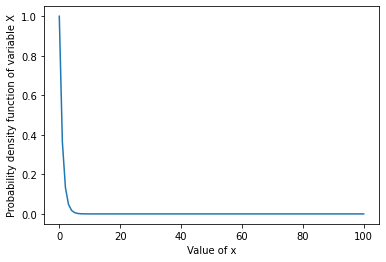
\includegraphics[width=\columnwidth]{solutions/2013/june/42/figures/figure2.png}
%     \caption{P.D.F. of X }
%     \label{june2013-42:june2013-42:fig:fig_label}
% \end{figure}
Let $f_X(x)$ denote the probability distribution function for random variable X.
\begin{align}
f_{X}(x)=
 \begin{cases} 
      \lambda_X  e^{-\lambda_X  x} & x \geq 0 \\
      0 & otherwise
 \end{cases}
\end{align}
Let $f_Y(y)$ denote the probability distribution function for random variable Y.
\begin{align}
f_{Y}(y)=
 \begin{cases} 
      \lambda_Y  e^{-\lambda_Y  y} & y \geq 0 \\
      0 & otherwise
 \end{cases}
 \end{align}
 Let $F_X(x)$ denote the cumulative distribution function for random variable X.
\begin{align}
F_{X}(x)=
 \begin{cases} 
      1-e^{-\lambda_X  x} & x \geq 0 \\
      0 & otherwise
 \end{cases}
\end{align}
Let $F_Y(y)$ denote the cumulative distribution function for random variable Y.
\begin{align}
F_{Y}(y)=
 \begin{cases} 
      1-e^{-\lambda_Y  y} & y \geq 0 \\
      0 & otherwise
 \end{cases}
 \end{align}
\begin{equation}\label{june2013-42:meanx}
    E(X)=\dfrac{1}{\lambda_X}
\end{equation}
\begin{equation}\label{june2013-42:meany}
    E(Y)=\dfrac{1}{\lambda_Y}
\end{equation}
From \ref{june2013-42:meanx} and \ref{june2013-42:meany},
\begin{equation}\label{june2013-42:lambda}
    \lambda_X = \lambda_Y = 1
\end{equation}
\begin{figure}[h]
    \centering
    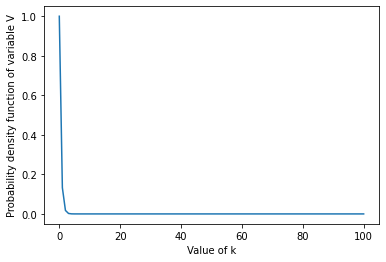
\includegraphics[width=\columnwidth]{solutions/2013/june/42/figures/figure.png}
    \caption{Parallel system}
    \label{june2013-42:fig:fig_label}
\end{figure}
Let Z be a random variable such that $Z=max(X,Y)$
\begin{align}
    P(Z\leq z) &= P(max(X,Y) \leq z)
    \\
    &=P(X\leq z,Y\leq z)
    \\
    &=P(X\leq z) P(Y\leq z)
    \\
    &=(F_X(z)-F_X(0)) (F_Y(z)-F_Y(0))
    \\
    &=1-e^{-(\lambda_X) z}-e^{-(\lambda_Y) z}+e^{-(\lambda_X+\lambda_Y) z}
\end{align}
$P(Z\leq z)$ denotes the probability that the system dies in the first $z$ seconds.\\
\begin{align}
    Expectation &= \int_{0}^{\infty}z \,d(P(Z\leq z))
    \\
\nonumber    &=\int_{0}^{\infty}z(\lambda_Xe^{-(\lambda_X) z}+\lambda_Ye^{-(\lambda_Y) z}\\
&-(\lambda_X+\lambda_Y)e^{-(\lambda_X+\lambda_Y) z}) \,dz
    \\
    &= \dfrac{1}{\lambda_X}+\dfrac{1}{\lambda_Y}-\dfrac{1}{\lambda_X+\lambda_Y}
\end{align}
From \ref{june2013-42:lambda}, 
\begin{equation}
    Expectation=\dfrac{3}{2}
\end{equation}
Therefore, option C correct.
